One example of a physical system that can be approximated by our first-order model is a automobile.  Let's consider how the speed of an automobile (the output) responds to changes in the gas petal (the input) as it moves in a constant direction.  The sketch if Figure~\ref{f:massd} illustrates this simplification of a complex physical system. 
\begin{figure}[hbt!]
\centering
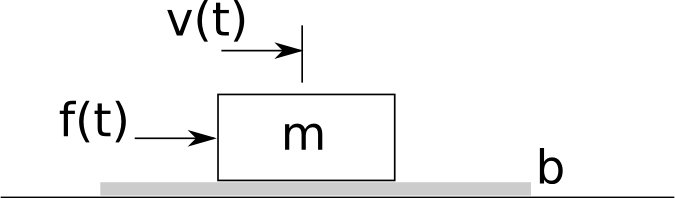
\includegraphics[width=\FigWidth\textwidth]{mass_damper.png}
\caption{Sketch of a simplified automobile model.  The point mass ($m$) moves to the right at a velocity ($v(t)$.  The input is a force ($f(t)$).  There is a drag force that resists the motion. }
\label{f:massd}
\end{figure}
Based on this sketch we can do things like draw a free-body-diagram and apply Newtonian principles to arrive at an equation of motion.  We might also make an ambitious simplifying assumption that the drag force that resists the motion of the mass is linearly related to the velocity, i.e., $f_{\mathrm{drag}}=b(v(t))$.  Then we could come up with an equation of motion
\begin{equation}
\label{e:car}
m\left(\dot{v}(t)\right) + b(v(t)) = f(t)
\end{equation}
where $m$ is the mass of the car, $v(t)$ is the speed, $\dot{v}(t)$ is the acceleration, $b$ is the coefficient of linear drag and $f(t)$ is the input force.  This equation of motion is our mathematical model
This equation has the same form (a first-order, linear, ordinary differential equation) as our first-order model~(\ref{e:first}).

This is meant to be an example of a model that is obviously wrong.  A physical automobile is a complex system with many, many degrees of freedom.  Our simplified model~(\ref{e:car}) is meant to do just one thing, allow us to predict how, in general, the speed of a car responds to changes in the throttle input.
